\chapter{Related Work}
\label{chapter:relatedwork}
\thispagestyle{myheadings}

\graphicspath{{2_RelatedWork/Figures/}}

\section{Memory Management in Rust}
\label{sec:history}

Each value in Rust has a variable called its owner. This owner has information about the value, such as location in memory, 
length and capacity of the value. This owner can live on the scope associated with its life time. When the owner goes out of it’s scope, 
the value will be dropped. When a value already assigned to a variable is assigned to another variable, if the value is allocated 
on heap its information is copied to the new owner and drop the old owner disabling old variable. Similar thing happens when we pass variable to parameter of function. 
After passing a variable to a parameter, all the information is copied to new owner through the parameter and old owner is no longer available. 
The new owner can only live in the function and the object will be dropped. In this case, we have no longer access to the object after the function. 
To avoid this, Rust has a concept called borrowing. We can set reference for the parameter of function and use the reference for operation within function and drop the reference, 
but not the ownership. 


\section{Spark and RDD Catching}
\label{sec:history}

Spark is one of the most used big data computing framework. Spark uses Resilient Distributed Datasets (RDDs) which implement in-memory data structures 
used to cache intermediate data across a set of nodes. This enables multiple rounds of computation on the same data, which is required for machine learning 
and graph analytics iteratively process the data. 

In RDD caching, there are different stages of caching, such as MEMOR\_YONLY and DISK\_ONLY. 
Currently, for very large data sets, we need to pay attention to garbage collection (GC) and OS page swapping overhead, 
because these could degrades execution time significantly. Therefore, DISK\_ONLY RDD caching can be better configuration in this case. 
However, writing and reading intermediate data among desk and memory could have bad effects for execution time, due to need of serialization and deserialization. 

\section{BLAS LAPACK}
\label{sec:history}

Basic Linear Algebra Subprograms (BLAS) are standard building blocks for basic vector and matrix operations. There are 3 levels of operation. The level 1 BLAS performs scalar, 
vector and vector-vector operations, the level 2 BLAS performs matrix-vector operation, and the level 3 BLAS performs matrix-matrix operation. 

LAPACK is developed on BLAS and has advanced functionalities such as LU decomposition and Singular Value Decomposition (SVD). Dense and banded matrices are handled, but not general 
sparse matrices. The initial motivation of development of LAPACK was to make the widely used EISPACK and LINPACK libraries run efficiently on shared-memory vector and parallel processors. 
LINPACK and EISPACK are inefficient because their memory access patterns disregard the multi-layered memory hierarchies of the machines, thereby spending too much time moving data. 
LAPACK addresses this problem by recognizing the algorithms to use block matrix operations, such as matrix multiplication, in the innermost loops. These block operations can be optimized for each architecture to account for the memory hierarchy, 
and so provide a portable way to achieve high efficiency on diverse modern machines. However, LAPACK requires that highly optimized block matrix operations be already implemented on each machine. 

ARPACK is also a collection of linear algebra subroutines which is designed to compute a few eigenvalues and corresponding eigenvectors from large scale matrix. 
ARPACK is based upon an algorithmic variant of the Arnoldi process called the Implicitly Restarted Arnoldi Method (IRAM). 
When the matrix is symmetric it reduces to a variant of the Lanczos process called the Implicitly Restarted Lanczos Method(IRLM). The Arnoldi process only interacts with the matrix via matrix-vector multiplies. 
Therefore, this method can be applied to distributed matrix operations required in big data analysis.


The original BLAS and LAPACK are written in Fortran90. Linear algebra library used for Spark is netlib-java, which is a Java wrapper library for Netlib, C API of BLAS and LAPACK. 
The reason why the developers addressed to use this package is that the BLAS and LAPACK are already bug free and implementing linear algebra library from scratch can usually buggy. 

However, the main advantage of use of BLAS and LAPACK is system optimized implementation. So if we implement original Fortran linear algebra library, it cannot perform as well as BLAS and LAPACK. 
And the performance would not be such different from one of implementation in Java or Rust.  If we want to test only memory management between Rust and Java, 
it can be enough implementation of linear algebra operation from  pure Java and Rust sacrificing the best performance taking advantage of system optimization. 


\section{Netlib-Java}
\label{sec:history}

Netlib-java is a Java wrapper of BLAS, LAPACK, and ARPACK. Netlib-java choose  implementation of linear algebra depending on installation of the libraries. 
First, if we have installed machine optimised system libraries, such as Intel MKL and OpenBLAS, netlib-java will use these as the implementation to use. 
Next, it try to load netlib references which netlib-java use CBLAS and LAPCKE interface to perform BLAS and LAPACK native call. 
The last option is to use f2j which is intended to translate the BLAS and LAPACK libraries from their Fortran77 reference source code to Java class files, 
instead of calling native libraries by using Java Native Interface (JNI). 

We can use JNI to call native libraries from Java. The JNI is a native programming interface which allows Java code that runs inside a Java Virtual Machine (VM) 
to interoperate with applications and libraries written in other programming languages. 

\section{Create Java interface of CBLAS with JNI}
\label{sec:history}
\begin{enumerate}
    \item Download BLAS and build using make file. In the figure2.1, the built file is libblas.a and the header file is blas.h.
    \item Download CBLAS and build using make file (I am not sure whether we should build archive file or shared library). In figure, the build file would be libcblas.a or libcblas.dylib and header file is cblas.h.
    \item Create java file which will be the Java interface of CBLAS.
    \item Compile java file with -h header flag to create class file (CBLASJ.class) and header file (CBLASJ.h).
\begin{lstlisting}[language=bash]
    $ javac -h . CBLASJ.java
\end{lstlisting}
    \item Create C file (CBLASJ.c) which will bind Java interface and CBLAS library. And compile it with JNI to create object file (CBLASJ.o).
\begin{lstlisting}[language=bash]
    $ gcc -c -fPIC -I${JAVA_HOME}/include -I${JAVA_HOME}/include/darwin CBLASJ.c
\end{lstlisting}
    \item Compile shared library linking library (libcblas.a or libcblas.dylib) object file (CBLASJ.o).
\begin{lstlisting}[language=bash]
    $ gcc -o libcblas.dylib (or libcblas.a) CBLASJ.o 
\end{lstlisting}
\end{enumerate}

\begin{figure}[htb]
    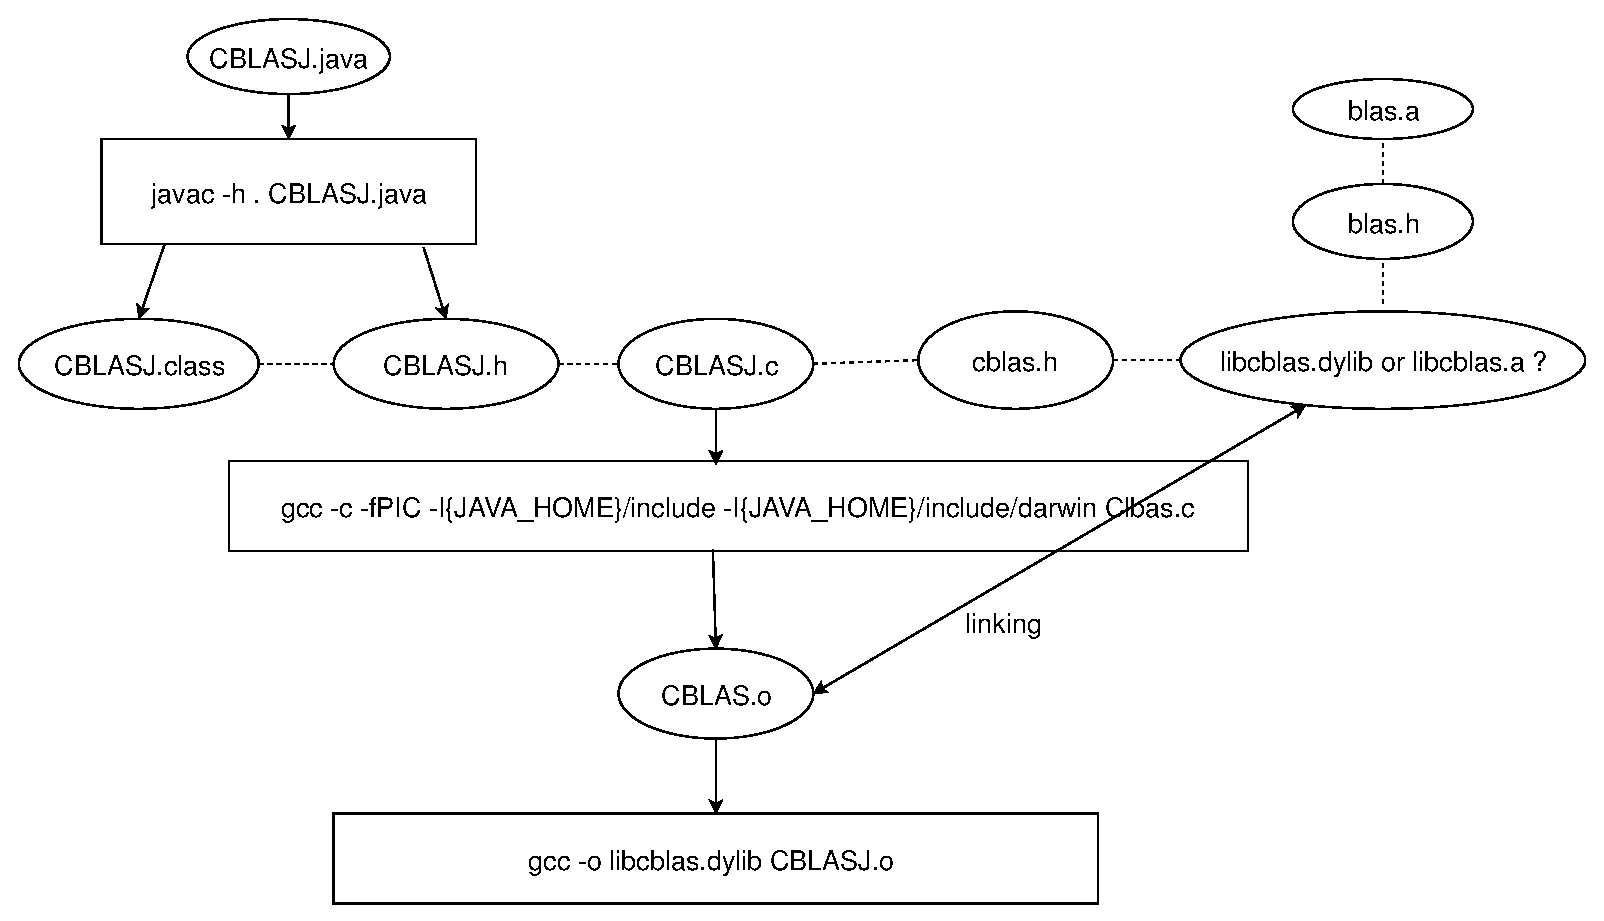
\includegraphics[width=15cm]{cblas_with_jni.eps}
    \caption{Integration of Native Methods }
    \label{fig:Sampling}
\end{figure}



\section{Matrix Computation and Optimization in Apache Spark}
\label{sec:history}

Matrix operation is a fundamental part of machine learning. Apache Spark provides implementation for distributed and local matrix operation. 
To translate single-node algorithms to run on a distributed cluster, Spark addresses separating matrix operations from vector operations and run matrix operations on the cluster, 
while keeping vector operations local to the driver. 

Spark changes its behavior for matrix operations depending on the type of operations and shape of matrices. For example, Singular Value Decomposition (SVD) for a square matrix is performed in distributed cluster, 
but SVD for a tall and skinny matrix is on a driver node. This is because the matrix derived among the computation of SVD for tall and skinny matrix is usually small so that it can fit to single node.

Spark uses ARPACK to solve square SVD. ARPACK is a collection of Fortran77 designed to solve eigenvalue problems. ARPACK is based upon an algorithmic variant of the Arnoldi process called the Implicitly Restarted Arnoldi Method (IRAM). 
When the matrix A is symmetric it reduces to a variant of the Lanczos process called the Implicitly Restarted Lanczos Method (IRLM). 
ARPACK calculate matrix multiplication by performing matrix-vector multiplication. So we can distribute matrix-vector multiplies, and exploit the computational resources available in the entire cluster. 
The other method to distribute matrix operations is Spark TFOCS. Spark TFOCS supports several optimization methods.

To allow full use of hardware-specific linear algebraic operations on single node, Spark uses the BLAS (Basic Linear Algebra Systems) interface with relevant libraries for CPU and GPU acceleration. 
Native libraries can be used in Scala are ones with C BLAS interface or wrapper and called through the Java native interface implemented in Netlib-java library and wrapped by the Scala library called Breeze. 
Following is some of the implementation of BLAS.

\begin{itemize}
    \item f2jblas -  Java implementation of Fortran BLAS
    \item OpenBLAS - open source CPU-optimized C implementation of BLAS
    \item MKL - CPU-optimized C and Fortran implementation of BLAS by Intel
\end{itemize}

These have different implementation and they perform differently for the type of operation and matrices shape. 
In Sark, OpenBlas is the default method of choice. BLAS interface is made specifically for dense linear algebra. 
Then, there are few libraries that efficiently handle sparse matrix operations.


\section{Memory Management of Java}
\label{sec:history}

Garbage Collection (GC) is a Java memory management method performed by JVM. 
GC tracks the state of objects on Java heap and triggers removal of unreferenced objects from memory. 

The Java heap structure is shown in Figure. It can be separated into three main parts where store objects for each corresponding generation: 
permanent generation, young generation, and old generation. The region for permanent generation stores metadata required by JVM to describe 
class and method used in application which will be permanently lived on the region of memory. 

The young generation of Java heap contains new objects allocated and aged. When the young generation fills up, this triggers minor GC. 
All of unreferenced objects will be removed from Java heap and remained objects will be aged and eventually promoted to the old generation.

The old generation is used to store long survived objects. Typically, a threshold is set for young generation object and when the age is met, 
the object will be moved to the old generation. Eventually, the old generation object also needs to be removed when the object is unreferenced. 
This is called major GC. The process of generational GC is shown in Figure.

\begin{figure}[htb]
    \includegraphics[width=15cm]{java_heap.eps}
    \caption{Java Heap Structure}
    \label{fig:Sampling}
\end{figure}


\begin{figure}[htb]
    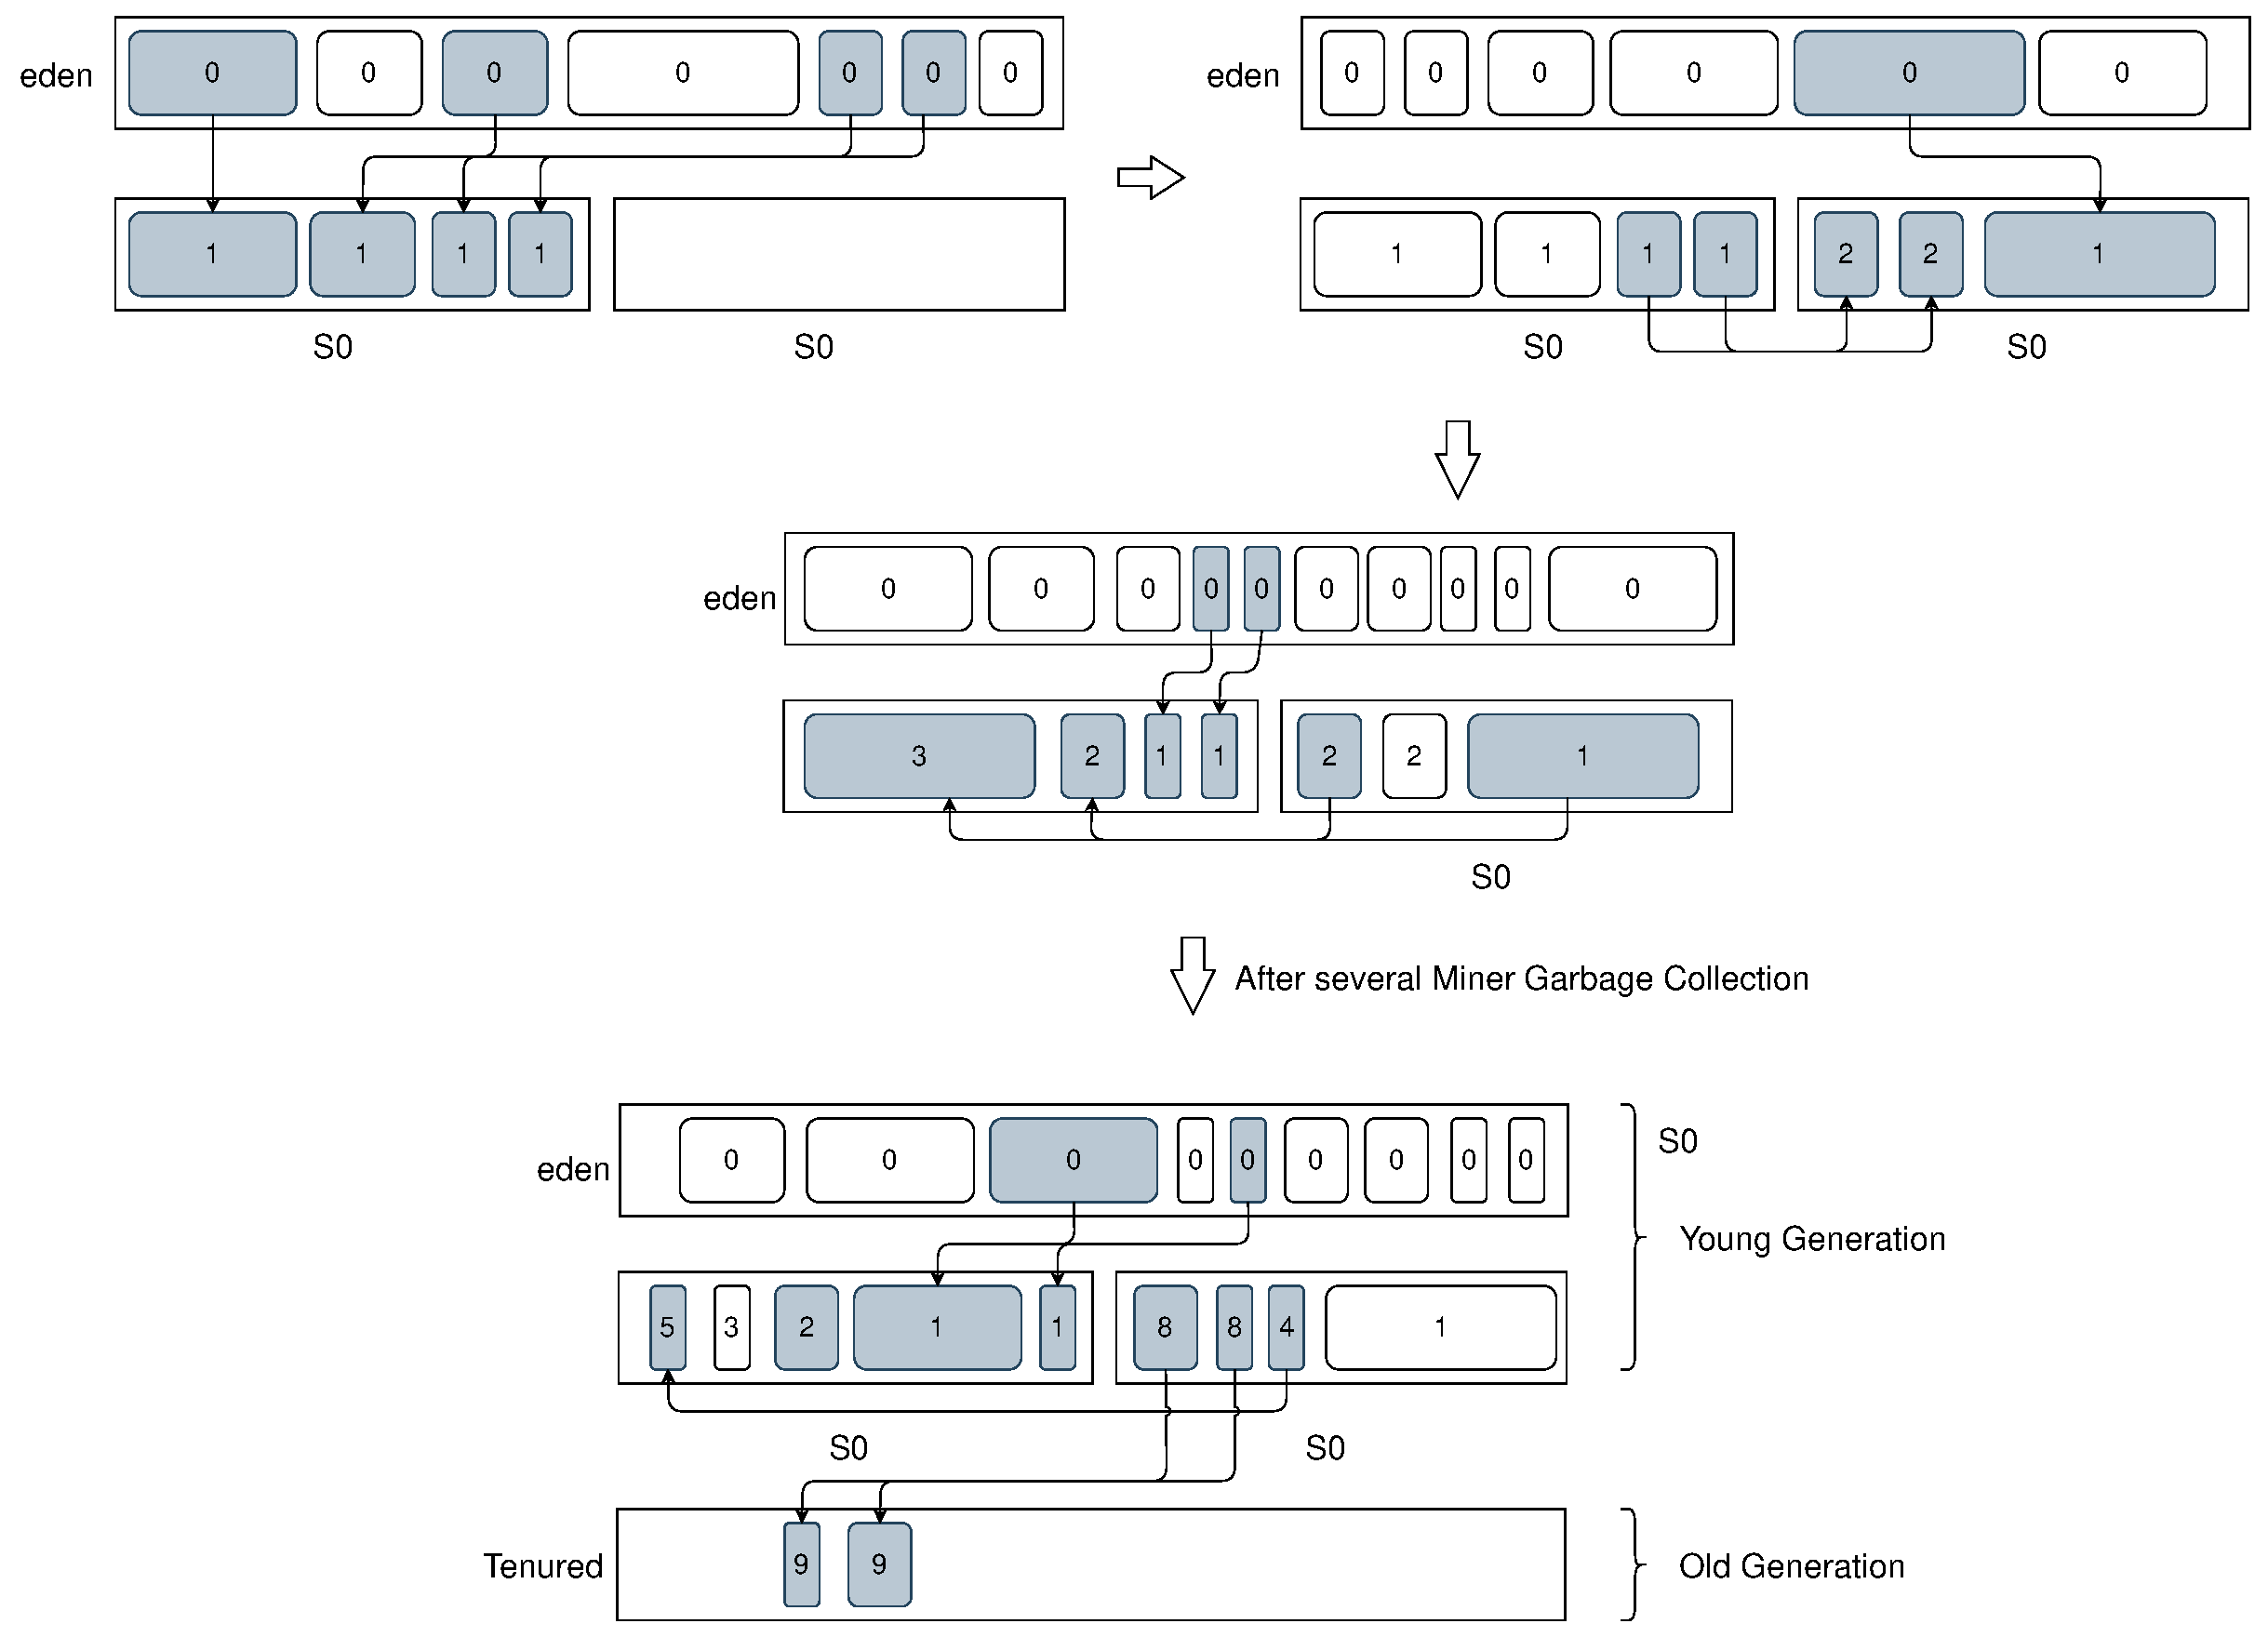
\includegraphics[width=15cm]{java_gc.eps}
    \caption{Java Garbage Collection}
    \label{fig:Sampling}
\end{figure}



\section{Memory Management of each Linear Algebra Library}
\label{sec:history}

The pure Java linear algebra library, such as La4j, EJML, and Apache Common Math, 
use normal GC performed by JVM to manage memory. This is because the implementation of these libraries are in purely Java.

Netlib-java, Jblas or other simple Java wrapper of BLAS, LAPACK, and ARPACK with Java Native Interface (JNI) use normal GC as well. 
This is because the native code deals with Java array by obtaining a reference to it. After the operation, 
the native method releases the reference to the Java array with or without returning new Java array or Java primitive type object. 

ND4J has two types of  its own memory management methods, GC to pointer of off-heap NDArray, and MemoryWorkspaces. 
ND4J used off-heap memory to store NDArrats, to provide better performance while working with NDArrays from vative code such as BLAS and CUDA libraries. 
Off-heap means that the memory is allocated outside of the Java heap so that it is not managed by the JVM’s GC. NDArray itself is not tracked by JVM, 
but its pointer is. The Java heap stores pointer to NDArray on off-heap. When a pointer is dereferenced, this pointer can be a target of JVM’s GC and when it is collected, 
the corresponding NDArray will be deallocated. When using MemoryWorkspaces, NDArray lives only within specific workspace scope. 
When NDArray leaves the workspace scope, the memory is deallocated unless explicitly calling method to copy the NDArray out of the scope.



\section{Experiment of Memory Allocation}
\label{sec:history}
This experiment is to test how static and dynamic memory allocation of Java and Rust behave. For the assessment, Element addition to ArrayList in the case of Java and Vector in the case of Rust 
is emploied here. These data stractures are resizable and we have control to set initial size. There are two parameters; initial size of ArrayList or Vector and thier final size after additions of elements. 
We are interested in the impact to memory allocation by initial allocation and expantion to runtime.

First, an ArrayList and an Vector are created with specified initial size. Then, in a loop, a element is added for each iteration until the size of the ArrayList or Vector get the specified final size. 
Each data structure has a different resizing strategy. When an ArrayList hits current limit of its size and expands the limit, it doubles the current size.  
While Vector does not have specific strategy for its resizing, the expantions of size of both ArrayList and Vector might affect the digradation of runtime performance.

To perform benchmarks, we use Java Microbenchamrk Hardness (JMH) for Java and Criterion for Rust. The benchmark time is calculated mean from several iterarions. 
We warm up before the execution. The parameters are set in combination of initial size, 10, 100, 1000, and 10000 and final size, 9, 99, 999, 9999. 
The results are shown in Figure 2-4 and 2-5. 

Discussions here are separated to two cases: when initial size is set bigger than final size and when final size is set bigger than initial size. 
For ArrayList in Java, it shows performance significant degradation when the initial size is bigger than final size. When we create ArrayList with intial size of 1000 and add 99 elements 
to the ArrayList, the the average execution time is 1125 ns. However, the average excution time when we create ArrayList with intial size of 100 and add 99 elements is 623 ns. 
This degration is caused by the cost of initializing the large array. On the other hand, Rust Vector does not have significant cost for the initialization of size compared to the cost of addition of elements. 
In the case of Vector with initial size of 1000 and add 99 elements to the Vector, the average excution is 320 ns. In the case of the initial size of 100 and 99 elements additions, 
the average excution is 279 ns. This is such small degradation compared to element addition in Vector. 

In ArrayList when the initial size is smaller than the final size, there can be degradation in performance. When its initial size and final size are set 100 and 999 respectively, 
the average execution time is 10884 ns. However when its initial size and final size are set 1000 and 999 respectively, the average execution time is 4250 ns. 
This result shows the degradation of in performance caused by the copy of existing elements into newly allocated array whose size is double of the last array.

This characteristic can be seen in the case of Vector in Rust. Vector with initial size 100 and final size 999 performs the average excution time 3514 ns, 
but one with initial size 1000 and final size 999 performs 2723 ns. When the Vector reachs its capacity, it allocates a larger buffer and copies the present elements to it.
This cost results in the degradation of the average excution time.

\begin{figure}[htb]
    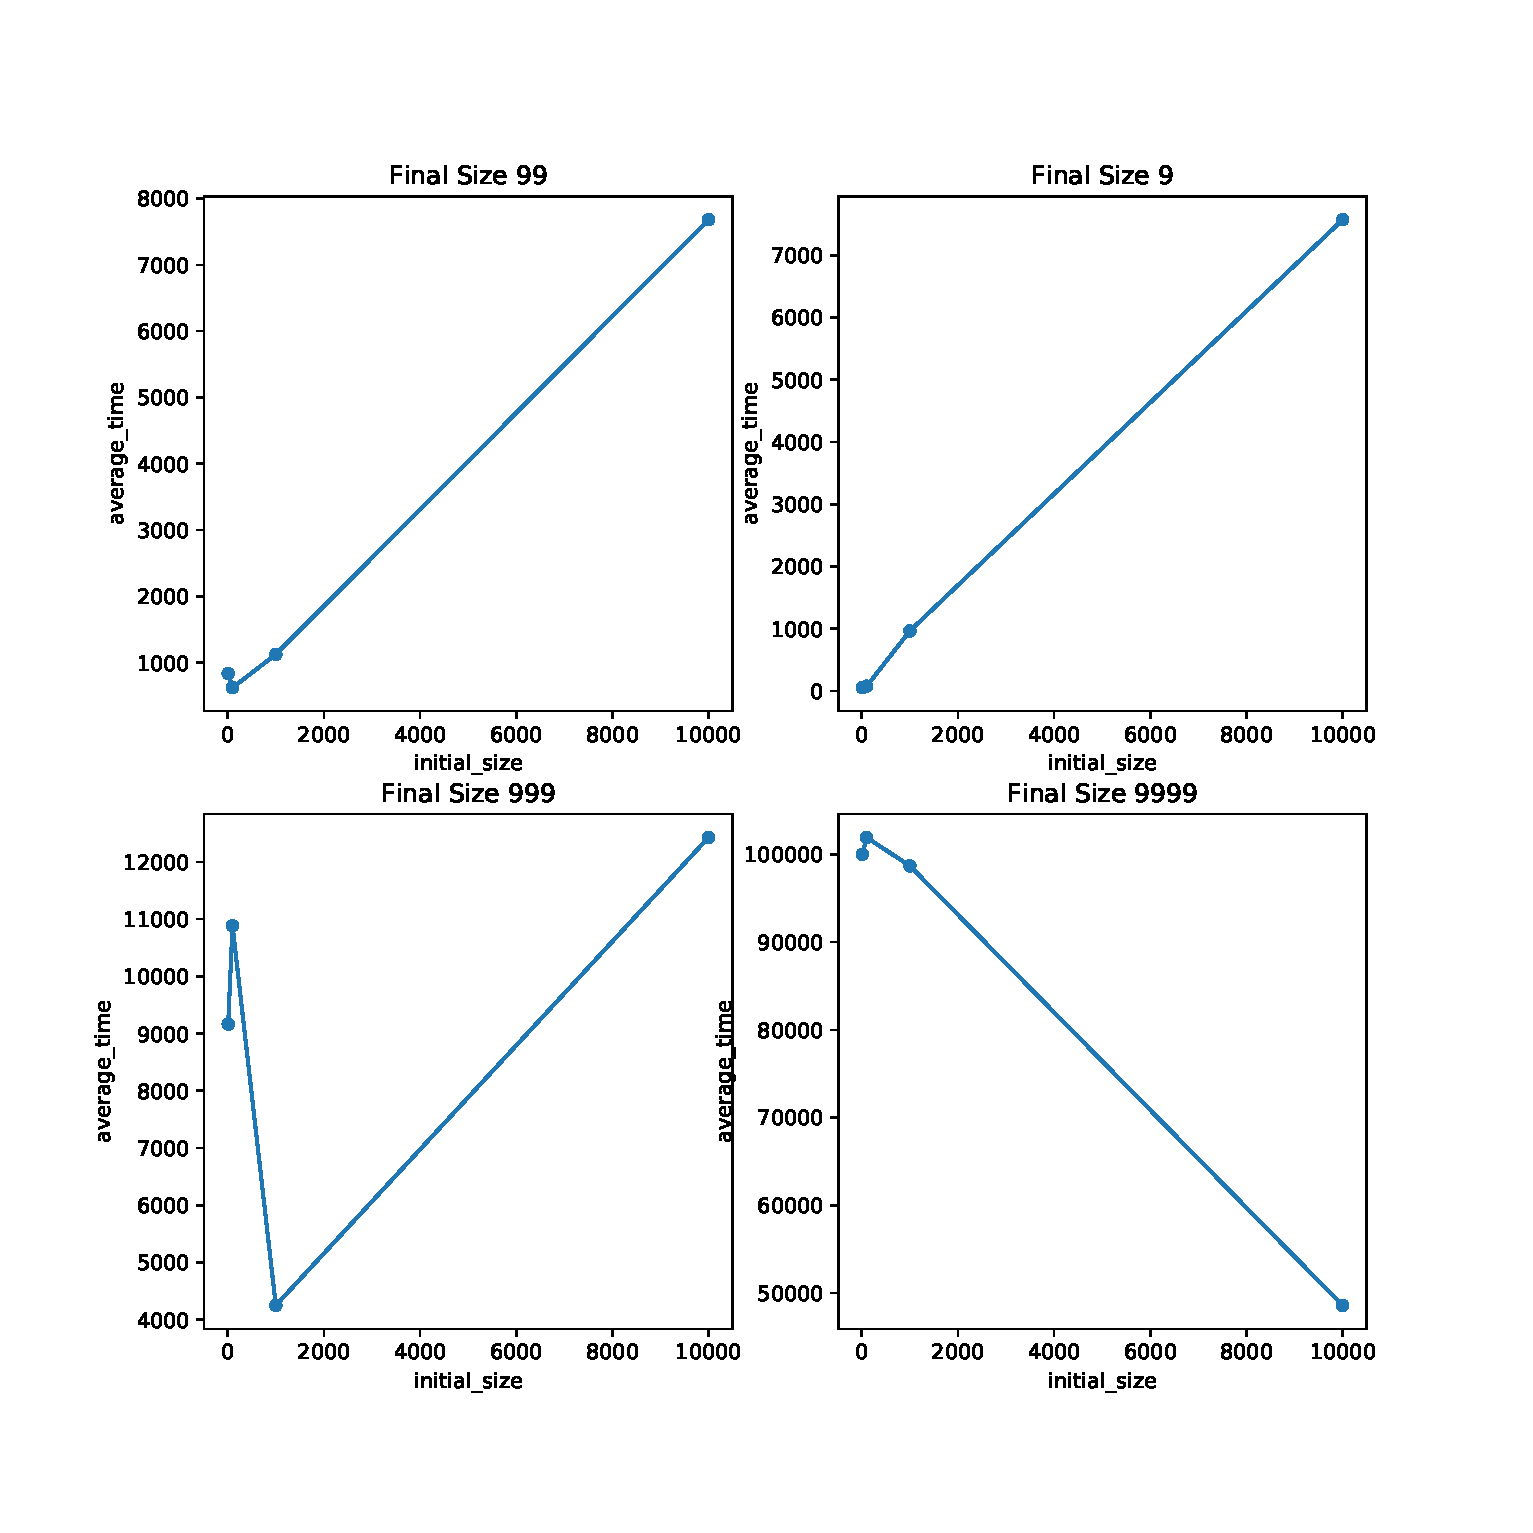
\includegraphics[width=15cm]{java_arraylist.eps}
    \caption{Memory allocation of ArrayList in Java}
    \label{fig:Sampling}
\end{figure}

\begin{figure}[htb]
    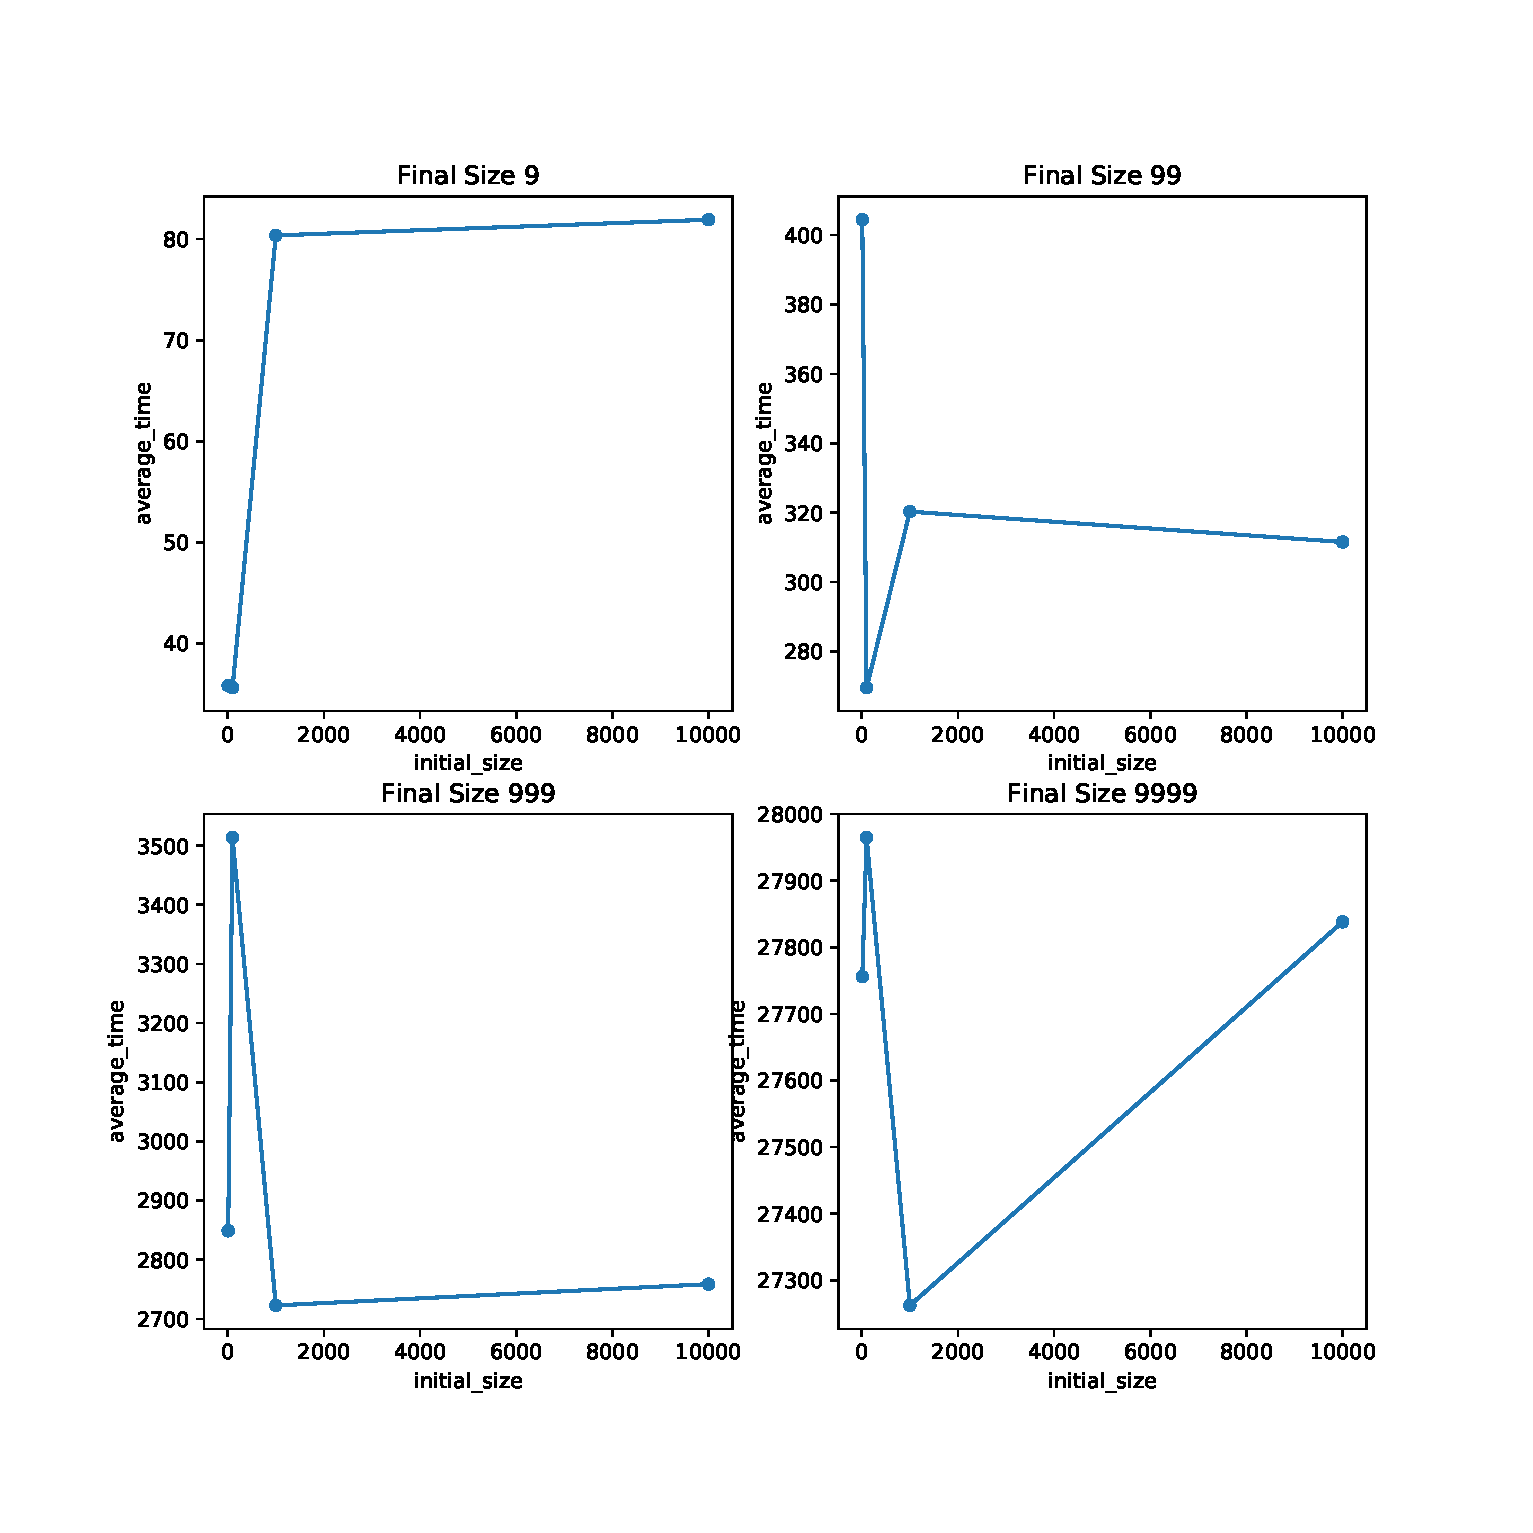
\includegraphics[width=15cm]{rust_vector.eps}
    \caption{Memory allocation of Vector in Rust}
    \label{fig:Sampling}
\end{figure}



\section{Experiment of Memory Allocation for Different Element Type.}
\label{sec:history}
This experiment is to test how static and dynamic memory allocation of Java and Rust behave. For the assessment, Element addition to ArrayList in the case of Java and Vector in the case of Rust 
is emploied here. These data stractures are resizable and we have control to set initial size. There are two parameters; initial size of ArrayList or Vector and thier final size after additions of elements. 
We are interested in the impact to runtime performance by initializing memory allocation and dynamicaly allocating memory space.

First, an ArrayList and an Vector are created with specified initial size. Then, in a loop, a element is added for each iteration until the size of the ArrayList or Vector get the specified final size. 
Each data structure has a different resizing strategy. When an ArrayList hits current limit of its size and expands the limit, it doubles the current size.  
While Vector does not have specific strategy for its resizing, the expantions of size of both ArrayList and Vector might affect the digradation of runtime performance.

Second, four types of element are used for elements addition to each data structure: integer, array of charactors, string, and Customer object. 
Assamption is that there would be different behavior between element additions of dynamically resizable and static size objects. 
Customer object has three fields. These fields are total order, weight of order, and zip code whose types are integer (i32 in rust), double (f32 in rust), and string respectively.
Figure 2-6 and 2-7 are representations of customer objects in Java and Rust.

Figure 2-10, 2-11, 2-12, and 2-13 represent the result of the experiments. For both data structures, integer elements addition shows the fastest runtime among all object types. 
This is because the compilers know each integer need 4 bytes to be stored in memory so that the space for memory that should be allocated is easily inspected. 
For the same reason, the initialization of data structures whose elements are integers alaways improves runtim performance.

The elements addition of strings and array of character behave similally among each languages. These two types of elements addition perform the similar speed and significantly slower than integer addition. 
Customer object addition is the slowest in Java. However, in Rust the addition of Customer object is the second fastest among all element typs.
The impacts of initialization of Java ArrayList vary among elemet types. On the other hand, the initailization Rust Vector always improves runtime performance for any of 4 types of elements addition.


\begin{figure}[htb]
    \begin{lstlisting}
        class Customer {
            int totalOrder;
            double weightOrder;
            String zipCode;
        }
    \end{lstlisting}
    \caption{Representation of Customer object in Java.}
    \label{fig:Sampling}    
\end{figure}

\begin{figure}[htb]
    \begin{lstlisting}
        struct Customer {
            total_order: i32,
            weight_order: f32,
            zip_code: String,
        }
    \end{lstlisting}
    \caption{Representation of Customer object in Rust.}
    \label{fig:Sampling}
\end{figure}

\begin{figure}[htb]
    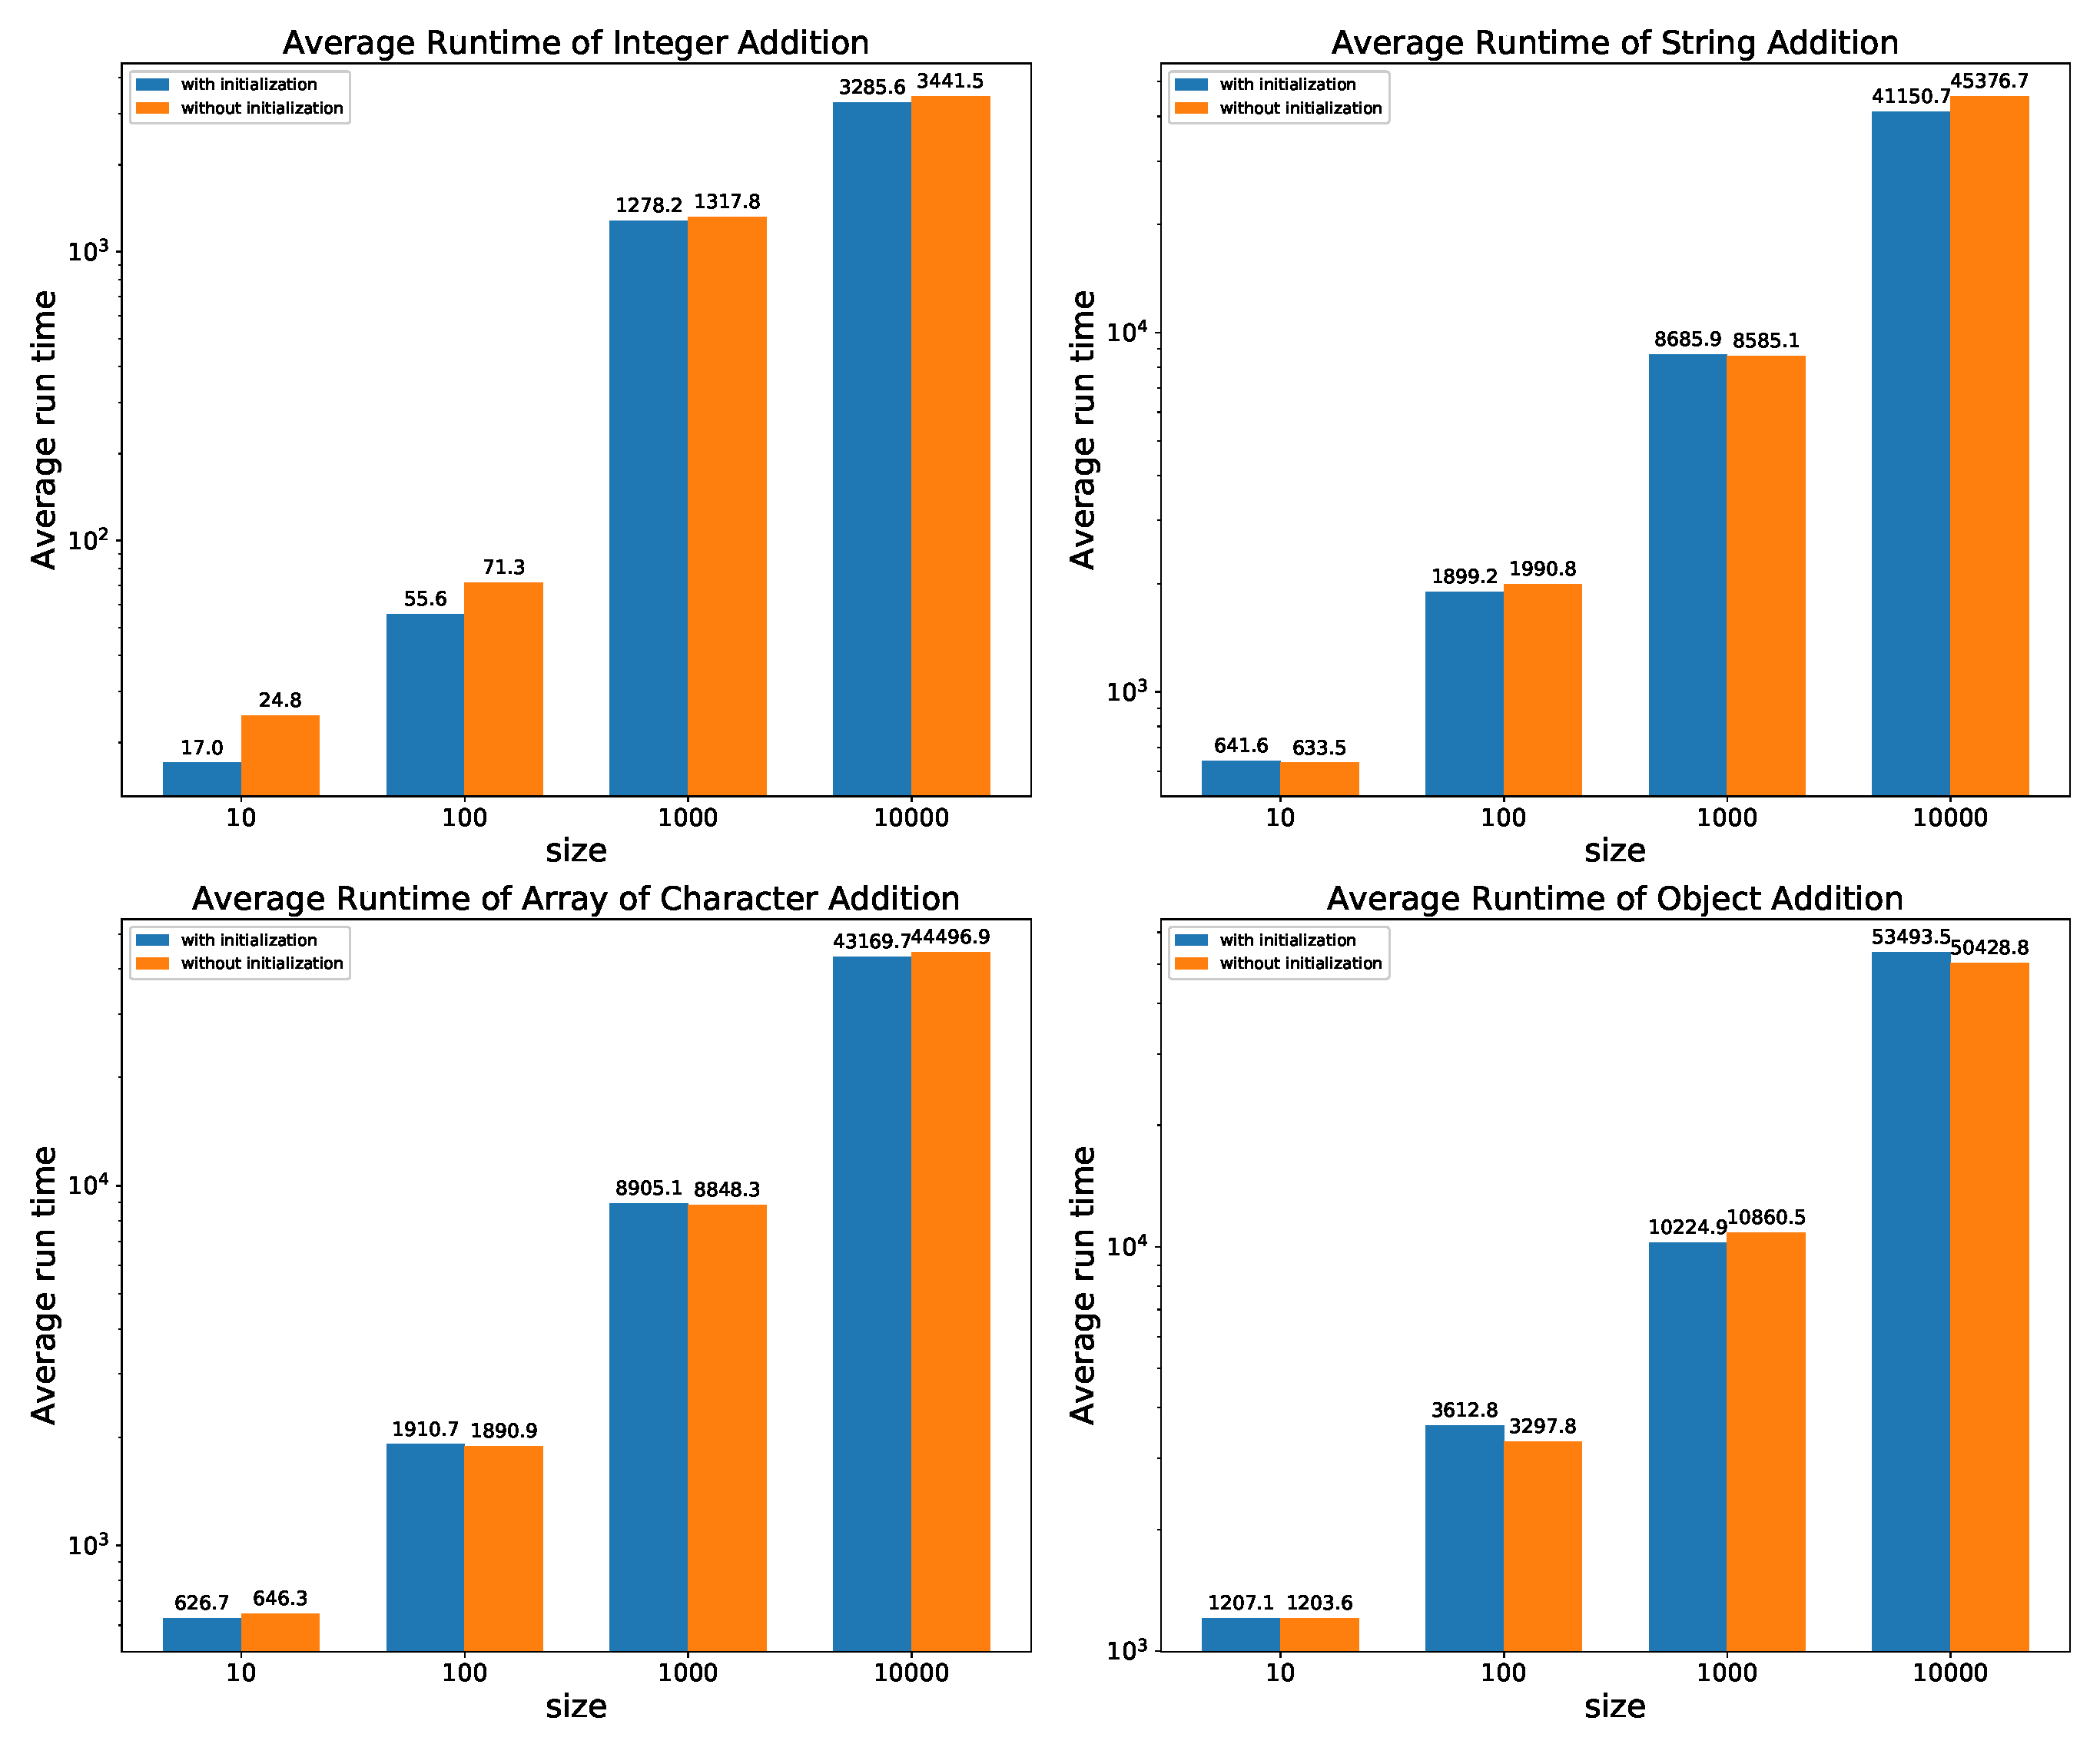
\includegraphics[width=15cm]{java_arraylist_log.eps}
    \caption{Memory allocation of Java ArrayList}
    \label{fig:Sampling}
\end{figure}

\begin{figure}[htb]
    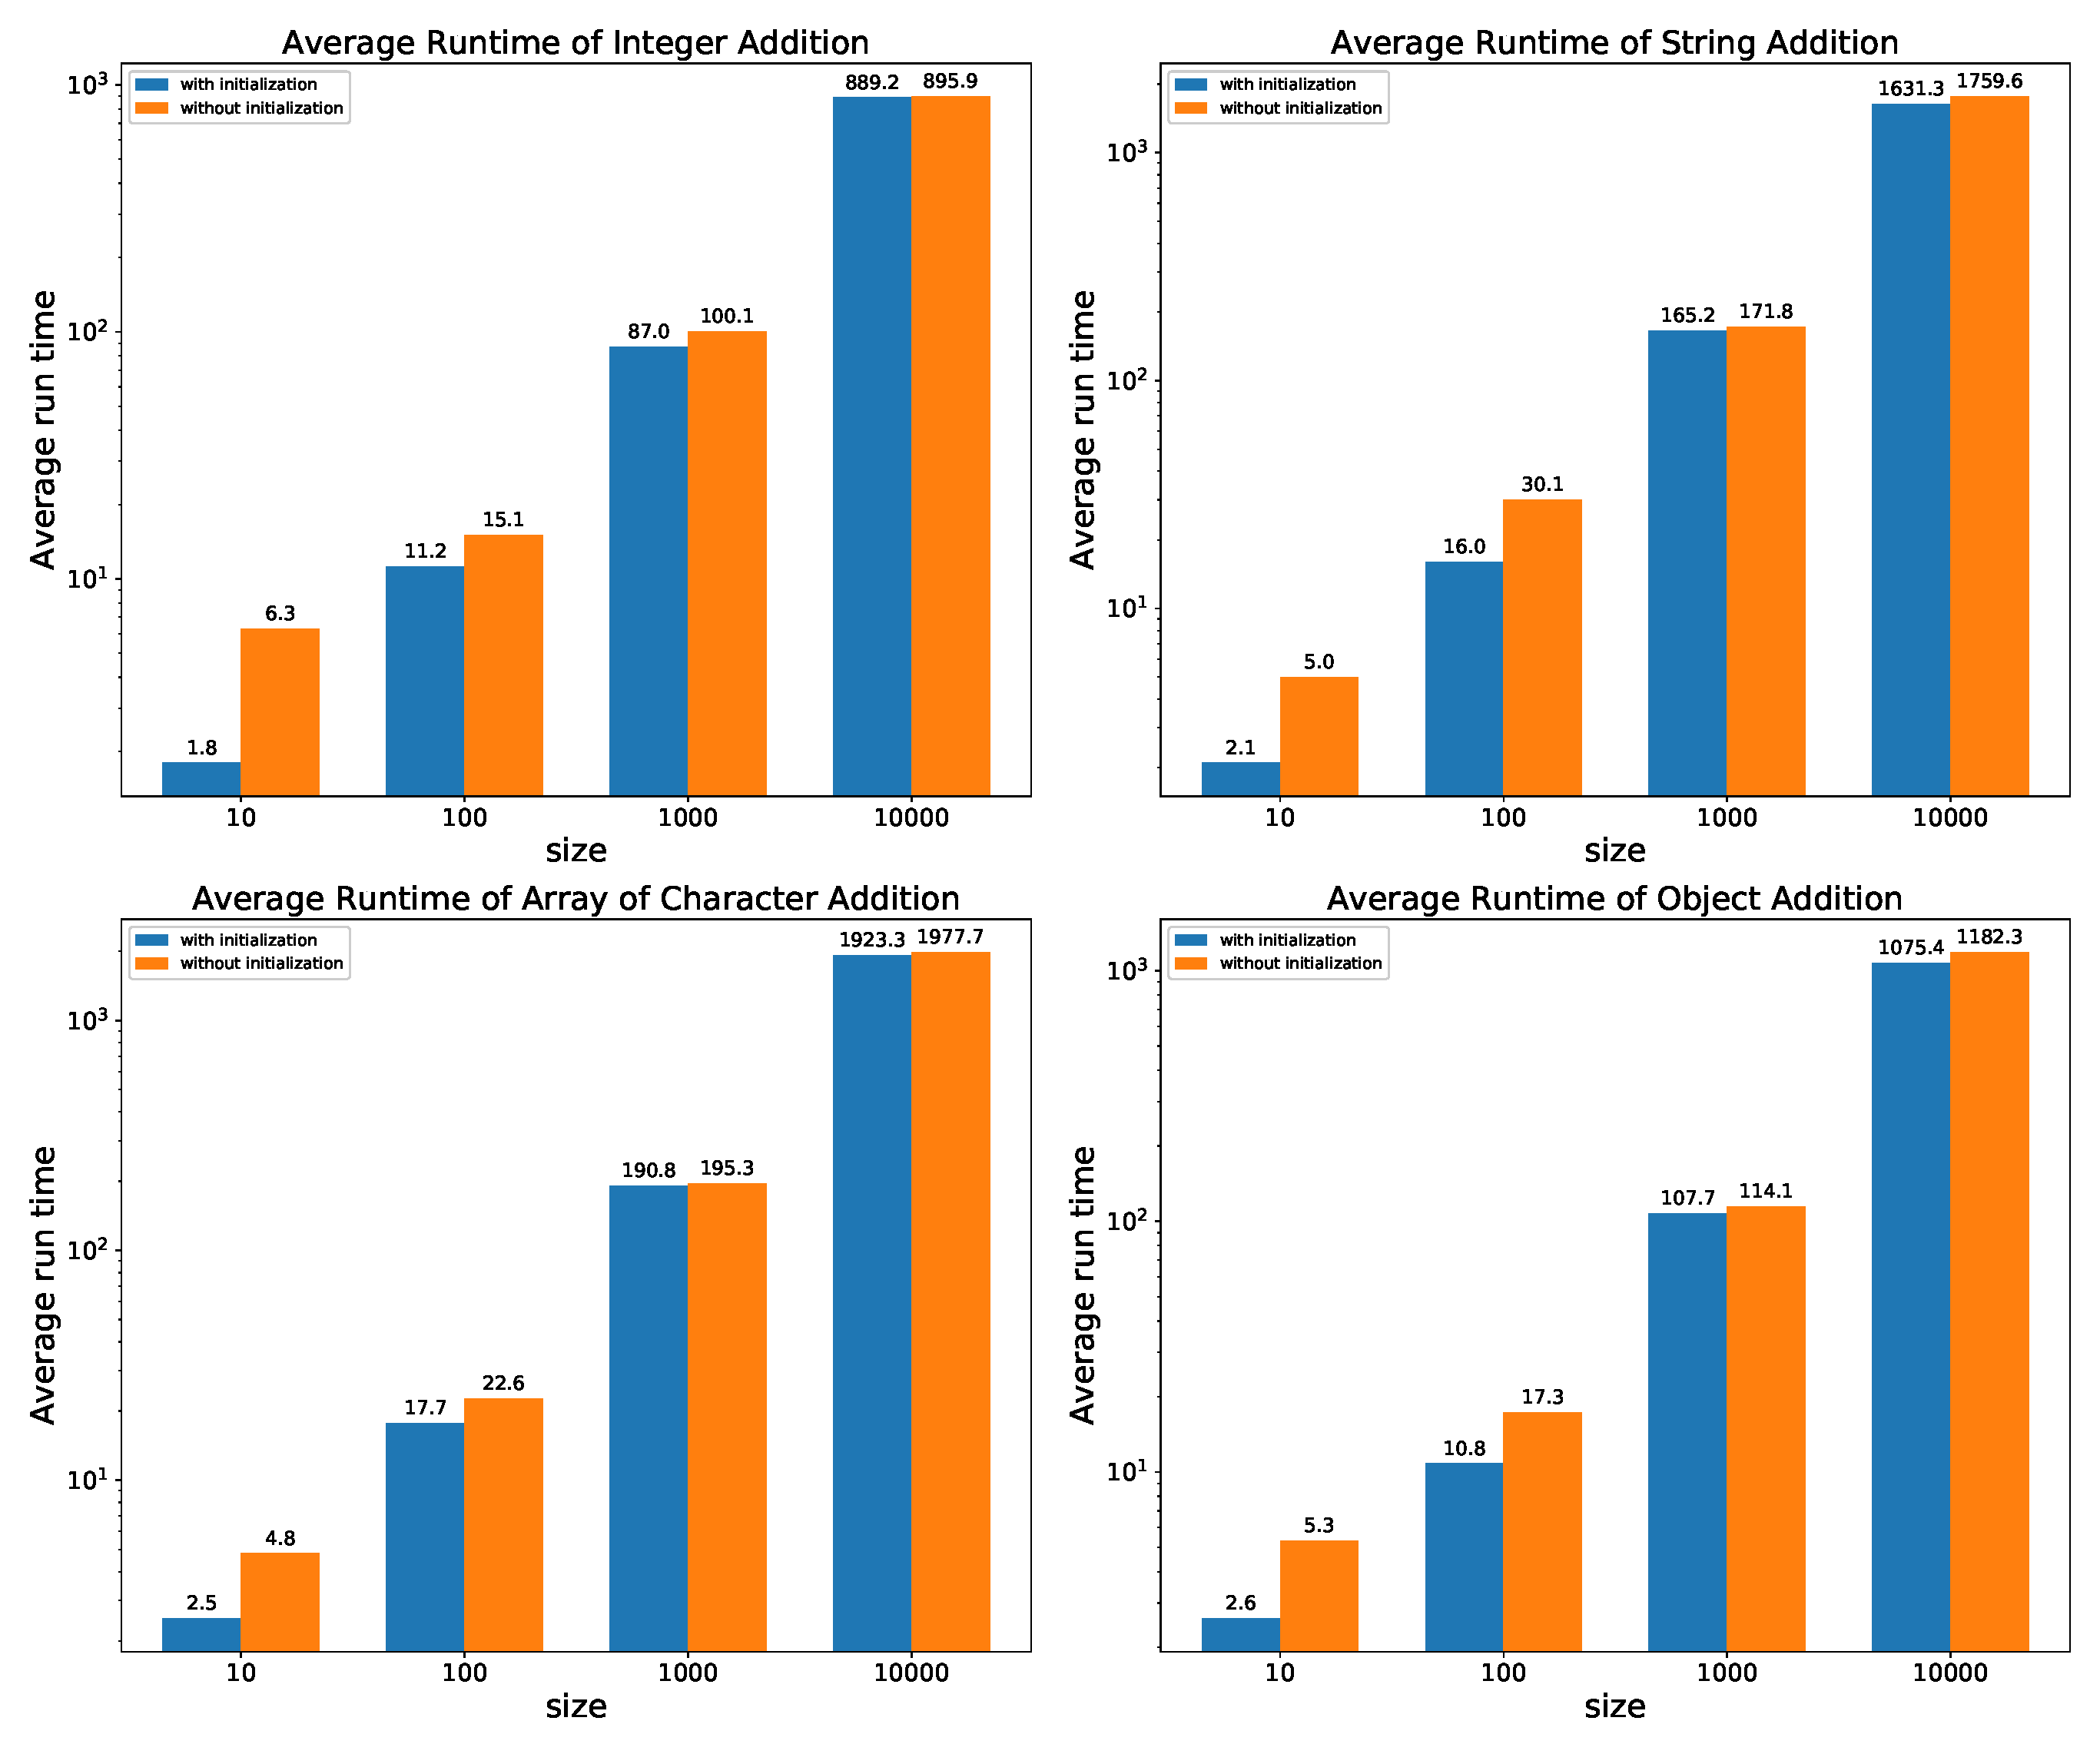
\includegraphics[width=15cm]{rust_vector_log.eps}
    \caption{Memory allocation of Rust Vector}
    \label{fig:Sampling}
\end{figure}


\begin{figure}[htb]
    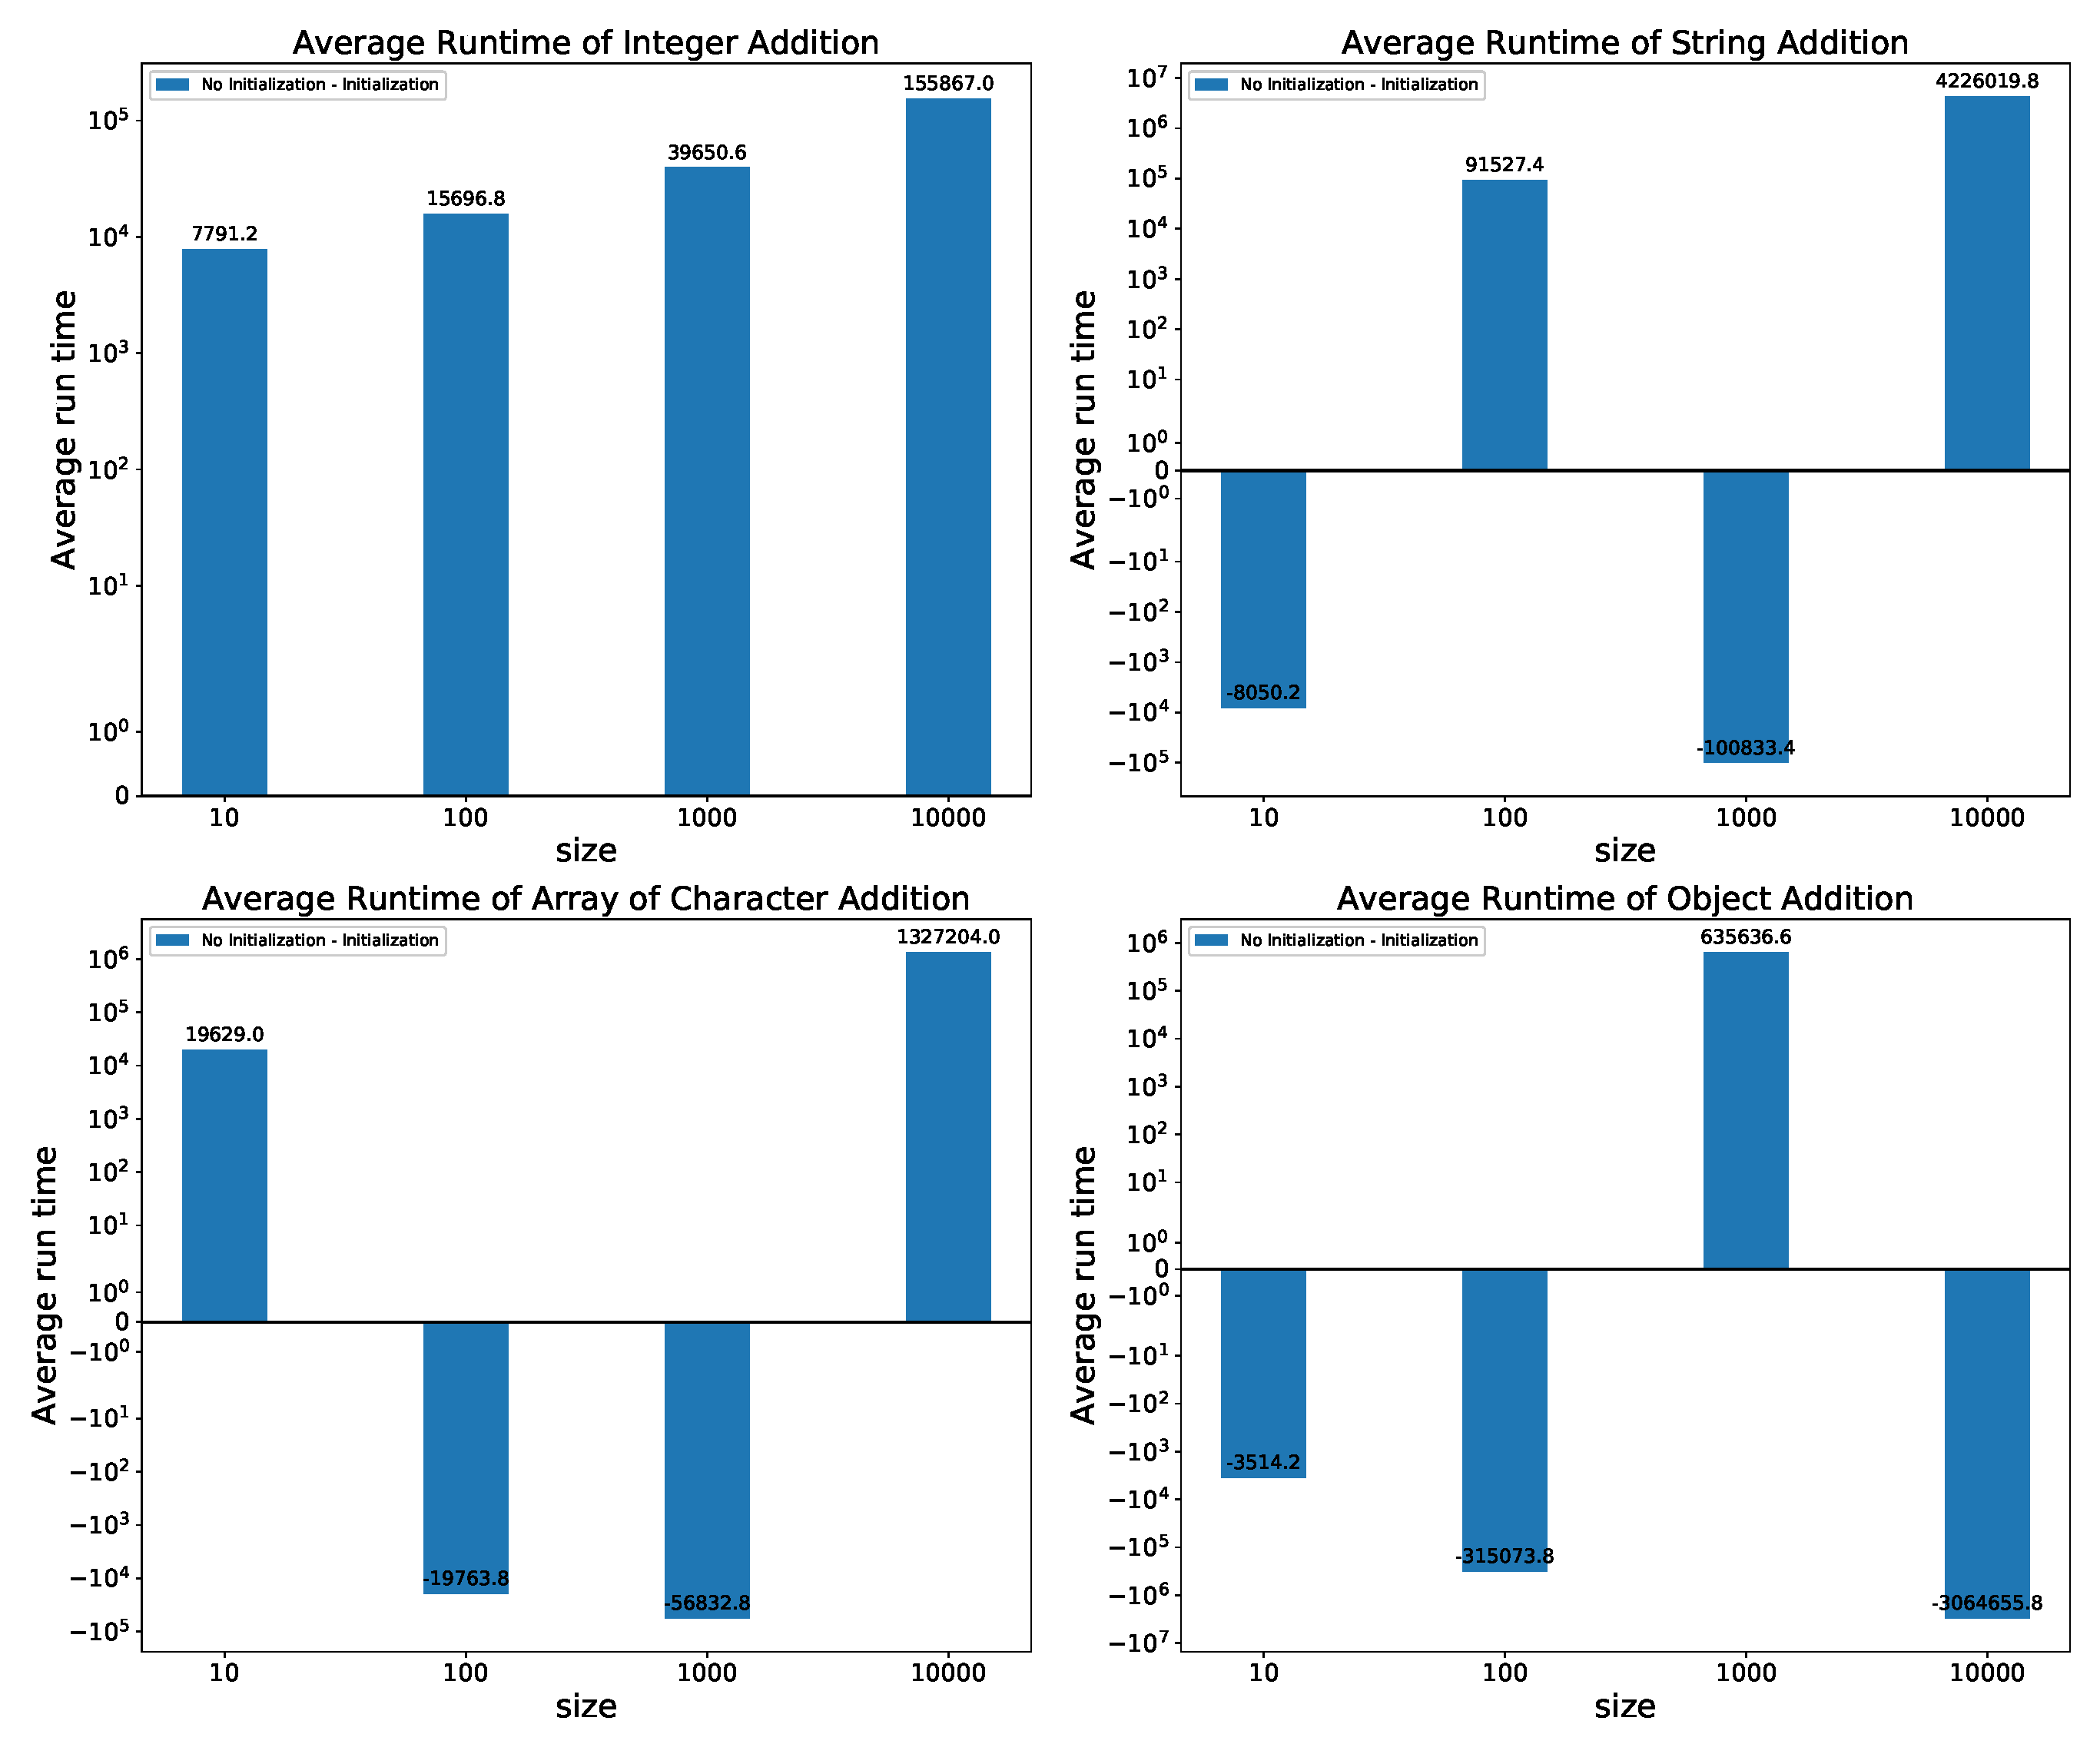
\includegraphics[width=15cm]{java_arraylist_difference.eps}
    \caption{Difference of Memory allocation of Java ArrayList between Non-initialization and Initialization}
    \label{fig:Sampling}
\end{figure}

\begin{figure}[htb]
    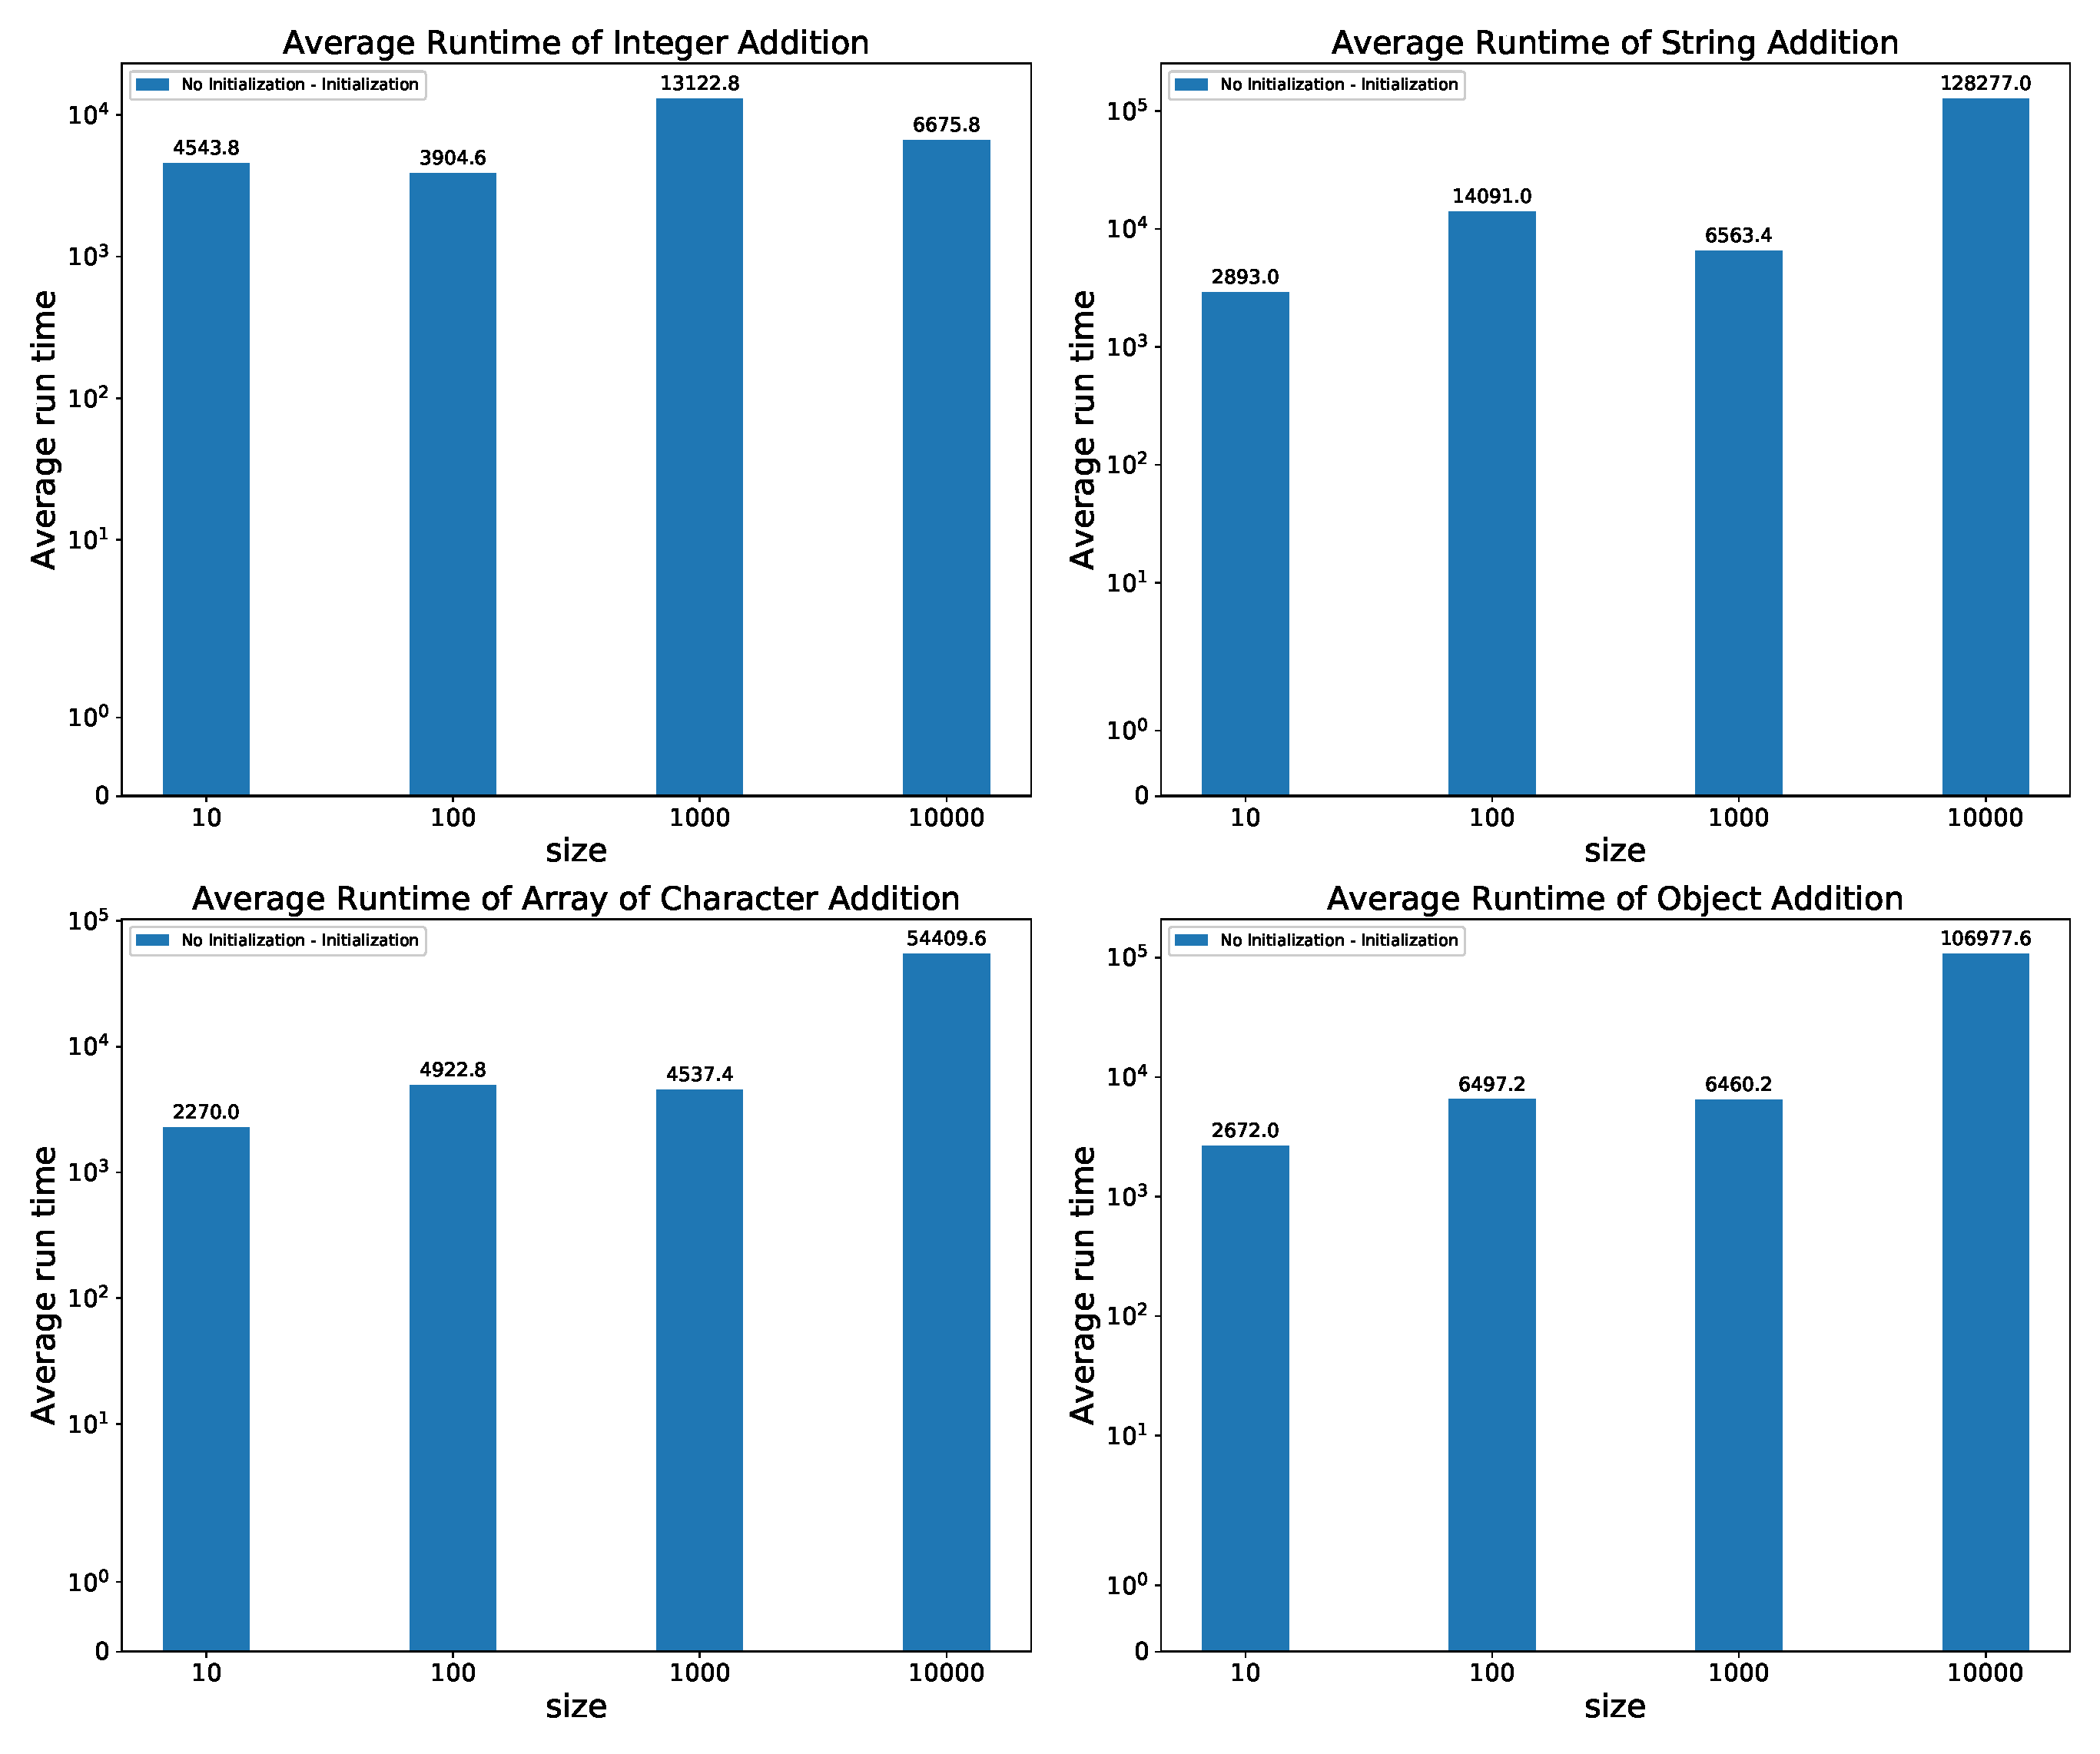
\includegraphics[width=15cm]{rust_arraylist_difference.eps}
    \caption{Difference of Memory allocation of Rust Vector between Non-initialization and Initialization}
    \label{fig:Sampling}
\end{figure}